\documentclass[%
  aspectratio=169,
  9pt,
  USenglish,
  titlegraphic, % store custom image to .images/titlegraphic
  affiliationintitlepagehead,
  progressbar,
%   affiliation,
]{beamer}

\usetheme{TUM}

\usepackage{tikz}  
\usepackage{tikz-3dplot} 
\usepackage{graphicx}
\usepackage{media9}
\usetikzlibrary{positioning}

\usepackage{amsmath}
\usepackage{booktabs}

% change the camera position
\tdplotsetmaincoords{45}{135}

\usepackage{tabularx}



\usepackage{animate}

\usepackage{pgfmath}
\newcommand\randmin{}
\newcommand\randmax{}
\newcommand\randmultof{}
\newcommand\setrand[4]%
{\def\randmin{#1}%
	\def\randmax{#2}%
	\def\randmultof{#3}%
	\pgfmathsetseed{#4}%
}
\newcommand\nextrand
{\pgfmathparse{int(int((rnd*(\randmax-\randmin+1)+\randmin)/\randmultof)*\randmultof)}%
	\xdef\thisrand{\pgfmathresult}%
}

%\usepackage[backend=biber]{biblatex}
%\addbibresource{bib/references.bib}

\newcommand{\wave}{
	\begin{tikzpicture}[xscale=.03,yscale=.1]
	\draw[-,fill=white] plot[domain=0:10*pi,smooth] (\x,{sin(\x r)});
	\end{tikzpicture}
}


\newcommand{\domain}[4]{
	%% spatial,spectral,temporal
	\draw[fill=#4, opacity=.2] (#1,0,0) -- (0,#2,0) -- (0,0,#3) -- (#1,0,0);
}


\newcommand{\radarwave}{
	\begin{tikzpicture}[xscale=.1,yscale=.2]
	\draw[-,fill=white] plot[domain=0:5*pi,smooth] (\x,{sin(\x r)});
	\end{tikzpicture}
}


\newcommand{\earth}{
	\begin{tikzpicture}[baseline=-.25em, inner sep=0]
	\node{
\includegraphics[width=8mm]{images/icons/earth}};
	\end{tikzpicture}
}

\newcommand{\sat}{
	\begin{tikzpicture}[baseline=-.25em, inner sep=0, remember picture]
	\node(sat)[rotate=270,anchor=center]{
\includegraphics[width=8mm]{images/icons/sat2}};
	\end{tikzpicture}
}


\usepackage[capitalize]{cleveref}
\usepackage[square,sort,comma,numbers]{natbib}

%% this hack seems to be nececessary due to incompatibilities of cvpr template and tikz... -> https://tex.stackexchange.com/questions/398223/tikz-gives-error-command-everyshipouthook-already-defined
%\makeatletter
%\@namedef{ver@everyshi.sty}{}
%\makeatother
%% hackend

\usepackage{tikz}
\usepackage{pgfplots}
\usetikzlibrary{positioning, calc,arrows,arrows.meta, fit}
%\usetikzlibrary{arrows.meta,calc,decorations.markings,math,arrows.meta}
\usepgfplotslibrary{groupplots}
\usepgfplotslibrary{fillbetween}
\usepgfplotslibrary{statistics} % provides boxplots
\usepackage{xfrac}

\newcommand{\tp}{tp}
\newcommand{\tn}{tn}
\newcommand{\fp}{fp}
\newcommand{\fn}{fn}


\usepackage{tumcolors}
\usepackage{tummath}
\newcommand{\yhat}{\hat{\V{y}}}
\newcommand{\ycorrect}{\hat{y}^+}
\newcommand{\thetadelta}{\V{\Theta}_\delta}
\newcommand{\biasdelta}{b_\delta}
\newcommand{\biasclass}{\V{b}_\text{c}}
\newcommand{\thetaclass}{\V{\Theta}_\text{c}}
\newcommand{\thetafeat}{\V{\Theta}_\text{feat}}
\newcommand{\fclass}{f_\text{c}}
\newcommand{\fdelta}{f_\delta}
\newcommand{\ffeat}{f_\text{feat}}
\newcommand{\f}{f}

\newcommand{\rvtime}{T_c} 
\newcommand{\xuptot}{\M{X}_{\rightarrow t}} 
\newcommand{\deltauptot}{\delta_{\rightarrow t}} 
\newcommand{\tstop}{\ensuremath{t_\text{stop}}}
\newcommand{\meantstop}{\ensuremath{\bar{t}_\text{stop}}}
\usepackage[super]{nth}
\usepackage{mathtools}

\definecolor{evalcolor}{HTML}{3F3F3F}
\definecolor{traincolor}{HTML}{B98951}
\definecolor{validcolor}{HTML}{3F4BBE}

\definecolor{fdlcolor}{HTML}{142737}

\usepackage{multimedia}

\colorlet{colortrain}{tumblue}
\colorlet{colorinfer}{tumblack}

\colorlet{earlinesscolor}{tumblue}
\colorlet{accuracycolor}{tumorange}

\colorlet{stdcolor}{tumbluelight}
\colorlet{mediancolor}{tumorange}
\colorlet{meancolor}{tumblue}

\colorlet{b1color}{tumdiagramaubergine}
\colorlet{b2color}{tumdiagramnavyblue}
\colorlet{b3color}{tumdiagramturquoise}
\colorlet{b4color}{tumdiagramgreen}
\colorlet{b5color}{tumdiagramlimegreen}
\colorlet{b6color}{tumdiagramyellow}
\colorlet{b7color}{tumdiagramsand}
\colorlet{b8color}{tumdiagramredorange}
\colorlet{b8Acolor}{tumdiagramred}
\colorlet{b9color}{tumblack}
\colorlet{b10color}{tumblue}
\colorlet{b11color}{tumdiagramdarkred}
\colorlet{b12color}{tumorange}

% atmospheric bands
\colorlet{b1color}{tumblack}%tumdiagramaubergine
\colorlet{b9color}{tumblack}%tumblack
\colorlet{b10color}{tumblack}%tumblue

%visisble bands
\colorlet{b2color}{tumblue}%tumdiagramnavyblue
\colorlet{b3color}{tumblue}%tumdiagramturquoise
\colorlet{b4color}{tumblue}%tumdiagramgreen

% near infrared bands
\colorlet{b5color}{tumdiagramred}%tumdiagramlimegreen
\colorlet{b6color}{tumdiagramred}%tumdiagramyellow
\colorlet{b7color}{tumdiagramred}%tumdiagramsand
\colorlet{b8color}{tumdiagramred}%tumdiagramredorange
\colorlet{b8Acolor}{tumdiagramred}%tumdiagramred

% SWIR bands
\colorlet{b11color}{tumorange}%tumdiagramdarkred
\colorlet{b12color}{tumorange}%tumorange

\colorlet{epsilon0color}{tumorange}
\colorlet{epsilon1color}{tumblue}
\colorlet{epsilon10color}{tumblack}

\colorlet{gridcolor}{tumblue}
\colorlet{activationcolor}{tumorange}

\colorlet{meadowcolor}{tumbluemedium}
\colorlet{wbarleycolor}{tumbluedark}
\colorlet{corncolor}{tumorange}
\colorlet{wheatcolor}{tumgreen}
\colorlet{sbarleycolor}{tumdiagramred}
\colorlet{clovercolor}{tumdiagramturquoise}
\colorlet{triticalecolor}{tumdiagramsand}

\tikzstyle{rnn}=[draw,circle, inner sep=.1em]
\tikzstyle{norm}=[rounded corners,draw]
\tikzstyle{annotation}=[rounded corners, fill=tumblue!20]
\tikzstyle{annot}=[-Stealth, thick]
\tikzstyle{infer}=[-stealth, shorten >=.0em, shorten <=.0em, colorinfer]
\tikzstyle{loss}=[fill=tumblue!10, rounded corners, font=\small]
\tikzstyle{grad}=[colortrain]

\newcommand{\ptoffset}{\varepsilon}

\tikzstyle{test} = [thick]
\tikzstyle{train} = [thin, dotted]

\usepackage[inline]{enumitem}
\setenumerate{label=(\roman*),itemsep=3pt,topsep=3pt}

\setlength{\belowcaptionskip}{-10pt}


\colorlet{traincolor}{tumbluelight}
\colorlet{validcolor}{tumbluedark}
\colorlet{evalcolor}{tumorange}

\colorlet{forwardcolor}{tumblue}
\colorlet{backwardcolor}{tumorange}

% defaultvalue -> might be replaced later
\colorlet{tensorcolor}{forwardcolor}

\colorlet{classcolor}{tumivory}
\colorlet{encodercolor}{tumblue}
\colorlet{encodercolor}{tumblue}
\colorlet{colorblue}{tumblue}
\colorlet{colororange}{tumorange}

\colorlet{colorclassone}{tumblue}
\colorlet{colorclasstwo}{tumblack}
\colorlet{colorclassthree}{tumorange}
\colorlet{colorclassfour}{tumgray}

\colorlet{frh01color}{tumgray}
\colorlet{frh02color}{tumorange}
\colorlet{frh03color}{tumblue}
\colorlet{frh04color}{tumblack}



%\usepackage{media9}

% notation
\newcommand{\MWeight}{\ensuremath{\M{W}}}
\newcommand{\VBias}{\ensuremath{\V{b}}}
\newcommand{\VInput}{\DataVec}
\newcommand{\VHidden}{\ensuremath{\V{h}}}
\newcommand{\FActivation}{\ensuremath{\sigma}}
\newcommand{\VCellState}{\ensuremath{\V{c}}}
\newcommand{\VForgetGate}{\ensuremath{\V{f}}}
\newcommand{\VModulationGate}{\ensuremath{\V{j}}}
\newcommand{\VInputGate}{\ensuremath{\V{i}}}
\newcommand{\VOutputGate}{\ensuremath{\V{o}}}
\newcommand{\concat}[2]{\left[#1 \parallel #2\right]}


\newcommand{\VResetGate}{\ensuremath{\V{r}}}
\newcommand{\VUpdateGate}{\ensuremath{\V{u}}}


%\usepackage{titlesec}
%\titlespacing{\section}{0pt}{10pt}{3pt}


\usetikzlibrary{3d}
\tikzstyle{perspective3d}=[
x={(0.5cm,0.5cm)}, y={(1cm,0cm)}, z={(0cm,1cm)}]


\usetikzlibrary{spy}

\usetikzlibrary{external,pgfplots.dateplot}

\usepackage[eulergreek]{sansmath}
\pgfplotsset{
	y tick label style={/pgf/number format/.cd,%
		scaled y ticks = false,
		set thousands separator={},
		fixed},
	x tick label style={/pgf/number format/.cd,%
		scaled x ticks = false,
		set decimal separator={,},
		fixed},
	tick label style = {font=\scriptsize\sansmath\sffamily},
	every axis label = {
		font=\scriptsize\sansmath\sffamily},
	every axis/.append style={
		axis lines=left, 
		enlargelimits, 
		thick},
	legend style = {font=\scriptsize\sansmath\sffamily, draw=none, rounded corners=0, fill opacity=.5, text opacity=1},
	label style = {font=\scriptsize\sansmath\sffamily},
	grid style={line width=.1pt, draw=gray!10},
	major grid style={line width=.2pt,draw=tumgraylight},
}

%\let\tempone\itemize
%\let\temptwo\enditemize
%\renewenvironment{itemize}{\tempone\addtolength{\itemsep}{-.5\baselineskip}}{\temptwo}

\tikzstyle{circ} = [circle, draw=white, fill=tumblue, inner sep=1pt]
\newcommand{\fcn}{
	\begin{tikzpicture}[scale=0.2, rotate=0, baseline=-.25em, inner sep=1pt]
	\node[circ](a0) at (0,-1){};
	\node[circ](a1) at (0,0){};
	\node[circ](a2) at (0,1){};
	
	\node[circ](b0) at (1,-0.5){};
	\node[circ](b1) at (1,0.5){};
	
	\draw[-] (a0) -- (b0);
	\draw[-] (a1) -- (b0);
	\draw[-] (a2) -- (b0);
	
	\draw[-] (a0) -- (b1);
	\draw[-] (a1) -- (b1);
	\draw[-] (a2) -- (b1);
	
	\end{tikzpicture}
}

\newcommand{\lfcn}[1]{
	\begin{tikzpicture}[scale=#1, rotate=0, baseline=-.25em, inner sep=1pt]
	\node[circle, draw=white, fill=tumblue, inner sep=3](a0) at (0,-1){};
	\node[circle, draw=white, fill=tumblue,  inner sep=3](a1) at (0,0){};
	\node[circle, draw=white, fill=tumblue,  inner sep=3](a2) at (0,1){};
	
	\node[circle, draw=white, fill=tumblue,  inner sep=3](b0) at (1,-0.5){};
	\node[circle, draw=white, fill=tumblue,  inner sep=3](b1) at (1,0.5){};
	
	\draw[-] (a0) -- (b0);
	\draw[-] (a1) -- (b0);
	\draw[-] (a2) -- (b0);
	
	\draw[-] (a0) -- (b1);
	\draw[-] (a1) -- (b1);
	\draw[-] (a2) -- (b1);
	
	\end{tikzpicture}
}

\newcommand{\hidden}[1]{
	\begin{tikzpicture}[scale=.1, baseline=-.25em]	
	%\draw[step=1.0,black,thin] (0,0) grid (#1,1);
	\foreach \i in {1,...,#1}{
		\node[circle, draw=white, fill=tumbluelight, inner sep=1pt] at (\i,0){};
	}
	\end{tikzpicture}
}

\newcommand{\drawvector}[1]{
	\begin{tikzpicture}[scale=.1, baseline=-.25em]	
	%\draw[step=1.0,black,thin] (0,0) grid (#1,1);
	\foreach \i in {1,...,#1}{
		\node[circ] at (\i,0){};
	}
	\end{tikzpicture}
}

%%%%%%%%%%%
%Coordinate Grid for easier placement of nodes
% \draw (0,1) to[grid with coordinates] (10,7);
%%%%%%%%%%%
\makeatletter
\def\grd@save@target#1{%
	\def\grd@target{#1}}
\def\grd@save@start#1{%
	\def\grd@start{#1}}
\tikzset{
	grid with coordinates/.style={
		to path={%
			\pgfextra{%
				\edef\grd@@target{(\tikztotarget)}%
				\tikz@scan@one@point\grd@save@target\grd@@target\relax
				\edef\grd@@start{(\tikztostart)}%
				\tikz@scan@one@point\grd@save@start\grd@@start\relax
				\draw[minor help lines] (\tikztostart) grid (\tikztotarget);
				\draw[major help lines] (\tikztostart) grid (\tikztotarget);
				\grd@start
				\pgfmathsetmacro{\grd@xa}{\the\pgf@x/1cm}
				\pgfmathsetmacro{\grd@ya}{\the\pgf@y/1cm}
				\grd@target
				\pgfmathsetmacro{\grd@xb}{\the\pgf@x/1cm}
				\pgfmathsetmacro{\grd@yb}{\the\pgf@y/1cm}
				\pgfmathsetmacro{\grd@xc}{\grd@xa + \pgfkeysvalueof{/tikz/grid with coordinates/major step}}
				\pgfmathsetmacro{\grd@yc}{\grd@ya + \pgfkeysvalueof{/tikz/grid with coordinates/major step}}
				\foreach \x in {\grd@xa,\grd@xc,...,\grd@xb}
				\node[anchor=north] at (\x,\grd@ya) {\pgfmathprintnumber{\x}};
				\foreach \y in {\grd@ya,\grd@yc,...,\grd@yb}
				\node[anchor=east] at (\grd@xa,\y) {\pgfmathprintnumber{\y}};
			}
		}
	},
	minor help lines/.style={
		help lines,
		step=\pgfkeysvalueof{/tikz/grid with coordinates/minor step}
	},
	major help lines/.style={
		help lines,
		line width=\pgfkeysvalueof{/tikz/grid with coordinates/major line width},
		step=\pgfkeysvalueof{/tikz/grid with coordinates/major step}
	},
	grid with coordinates/.cd,
	minor step/.initial=.2,
	major step/.initial=1,
	major line width/.initial=2pt,
}
\makeatother

\newcommand\tikzmark[1]{
	\tikz[remember picture,overlay] \coordinate (#1);
}
\newcommand\remembername[2]{
	\begin{tikzpicture}[inner sep=0]
		\node(#2){#1};
	\end{tikzpicture}
%	\tikz[remember picture,overlay] \coordinate (#1);
}

\newcommand{\bluebf}[1]{{\color{tumblue}\textbf{#1}}}
\newcommand{\orangebf}[1]{{\color{tumorange}\textbf{#1}}}

\setbeamertemplate{blocks}[rounded][shadow=false]

\title{Multi-temporal Earth Observation}
\subtitle{Learning Vegetation Models}
\author[M. Rußwurm]{Marc Rußwurm}
\institute[TUM]{Technical University of Munich, Germany\\
                Remote Sensing Technology}
\date{\today}

\begin{document}
\begin{frame}[t]
  \titlepage
\end{frame}

\begin{frame}
  \frametitle{The bigger Picture}
  \begin{itemize}
  	\item end-to-end learning
  	\item generalizability
  	\item learning of a vegetation model
  \end{itemize}
\end{frame}

\begin{frame}
\frametitle{Optical Satellites}
\begin{columns}
	\column{.5\textwidth}
	
	
	\begin{itemize}[itemsep=.5em]
		\item<1-> Sensor measures \textbf{Digital Numbers} $\text{DN}(\lambda)$ for each wavelength $\lambda$. 
		\item<2-> \textbf{Digital Numbers} are normalized to \textbf{Radiance} 
		$L(\lambda), \left[\frac{W}{\text{sr}m^2}\right]$ by gain and offset calibration.
		\item<3-> Radiance is normalized to \textbf{top-of-atmosphere reflectance} $\rho(\lambda)$
		%		\item<4-> \textbf{Bottom-of-atmosphere reflectances} are reconstructed using a functional model of the atmosphere.
	\end{itemize}
	
	%	Radiance $R_\lambda$ from measured Digital Numbers via calibrated gain $\alpha$ and offset $\beta$
	%	\begin{equation*}
	%		L_\lambda = \alpha \text{DN}_\lambda + \beta, \left[\frac{W}{\text{sr}m^1}\right]
	%	\end{equation*}
	%	
	%	top-of-atmosphere reflectance $\rho_\lambda$ as normalized Radiance $R_\lambda$ with solar 
	%	\begin{equation*}
	%	\rho_\lambda = \frac{L_\lambda}{\cos(\varphi_\text{sun})}
	%	\frac{
	%		\pi d^2
	%	}
	%	{
	%		E_\text{sun}(\lambda)
	%	}
	%	\end{equation*}
	%	
	%	\vspace{1em}
	%	
	%	\begin{itemize}
	%		\item measured radiance $L(\lambda)$
	%		\item solar irradiance $E_\text{sun}(\lambda)$
	%		\item solar zenith angle $\varphi_\text{sun}$
	%		\item squared Earth-Sun distance $d$ in AU
	%	\end{itemize}
	
	
	\column{.5\textwidth}
	
	
	\begin{tikzpicture}
	
	
	%	\draw [black,dotted, fill=tumbluelight,domain=110:70] plot ({13*cos(\x)}, {13*sin(\x)-12.8});
	\draw [fill=tumivory,domain=110:70] plot ({10*cos(\x)}, {10*sin(\x)-10});
	%	\draw [fill=tumbluelight,domain=110:70] plot ({12*cos(\x)}f, {12*sin(\x)-10});
	
	
	\node(sun) at (-2,2) {
\includegraphics[width=10mm]{images/icons/sun}};
	\node[rotate=130,anchor=center](sat) at (2,2) {
\includegraphics[width=10mm]{images/icons/sat2}};
	
	\node(px) at ({10*cos(90)}, {10*sin(90)-10.1}){
		\begin{tikzpicture}[xscale=.5,yscale=.25]
		\draw[fill=tumbluelight] (0,0) -- (1,0) -- (2,1) -- (1,1) -- (0,0);
		\end{tikzpicture}
		%
\includegraphics[width=5mm]{images/icons/house}
	};
	
	\draw[-stealth] (sun) -- node[midway,sloped]{\wave} (px);
	\draw[-stealth] (px) -- node[midway,sloped]{\wave} (sat);
	
	\visible<3->{\draw[-stealth] (sun) -- node[midway,sloped]{\wave} (sat);
		\draw[draw=tumgray] (px) -- node[at end,left]{$\varphi_\text{sun}$} ++(0,1.4); 
		\draw [draw=tumgray, domain=130:90] plot ({1*cos(\x)}, {1*sin(\x)});
	}
	
	\node[above=.5em of sun]{$E_\text{sun}(\lambda)$};
	\visible<1>{\node[above=4em of sat]{$DN(\lambda)$};}
	\visible<2>{\node[above=4em of sat]{$L(\lambda)$};}
	\visible<3>{\node[above=4em of sat]{$\rho_\text{toa}(\lambda)$};}
	%	\visible<4>{\node[above=4em of sat]{$\rho_\text{boa}(\lambda)$};}
	
	%		\draw[red] (0,0) sin (1,2);
	
\end{tikzpicture}
\end{columns}
\end{frame}

\begin{frame}
\frametitle{Acquired in regular time intervals}
\framesubtitle{Sentinel 2 Satellite}

%	\includemovie[
%	poster,
%	text={\small(Loading Circle-m-increase3.mp4)}
%	]{6cm}{6cm}{images/s2orbits.mp4}
%	
%	\movie{loaded}{images/s2orbits.avi}

\begin{columns}
\column{.5\textwidth}

\Large
\begin{itemize}
\item<1-> polar sun-synchronous orbit
\item<2-> single orbit circa 100 minutes
\item<3-> revisit same location after 5 days
\item<4-> acquisition stripe of 290km width
\item<5-> 13 spectral bands
\item<6-> ground resolution 10-60m
\item<7-> global coverage and free of charge
\end{itemize}

\column{.5\textwidth}
%		\only<1>{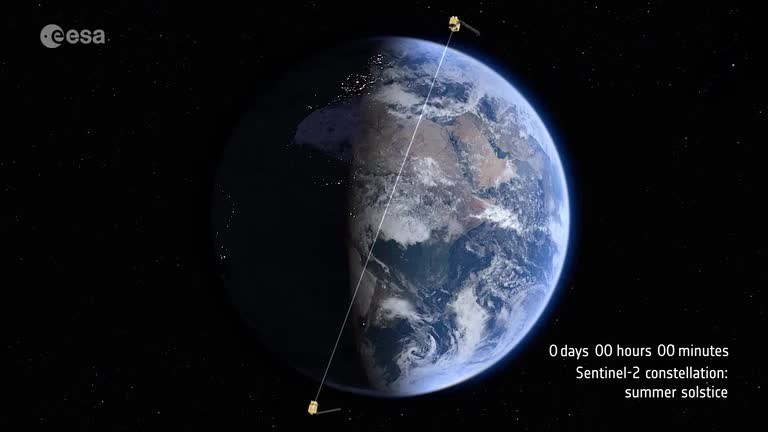
\includegraphics[width=\textwidth]{images/s2orbits/1}}
%		\only<2>{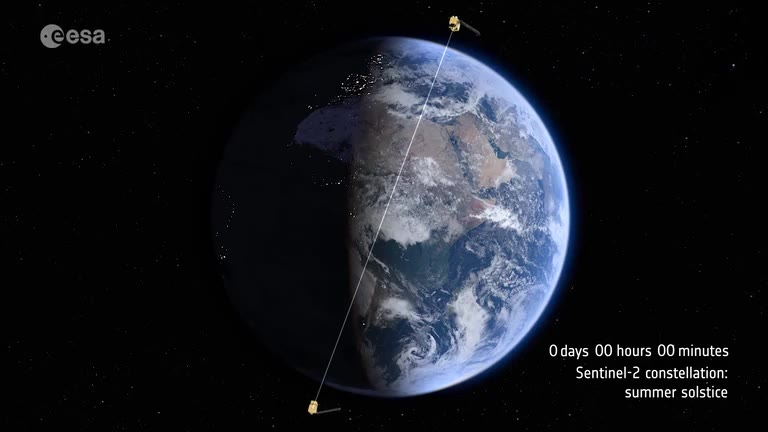
\includegraphics[width=\textwidth]{images/s2orbits/2}}
%		\only<3>{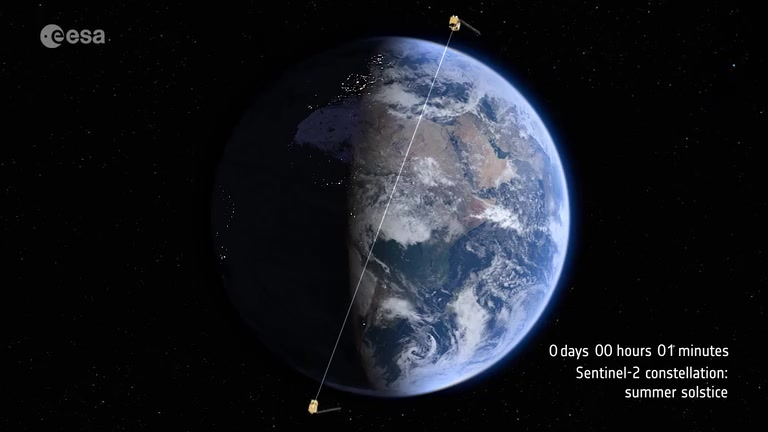
\includegraphics[width=\textwidth]{images/s2orbits/3}}
\only<1>{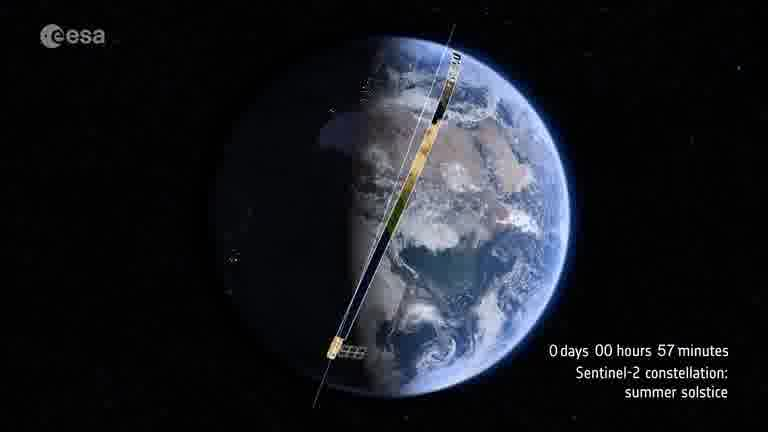
\includegraphics[width=\textwidth]{images/s2orbits/14}}
\only<2>{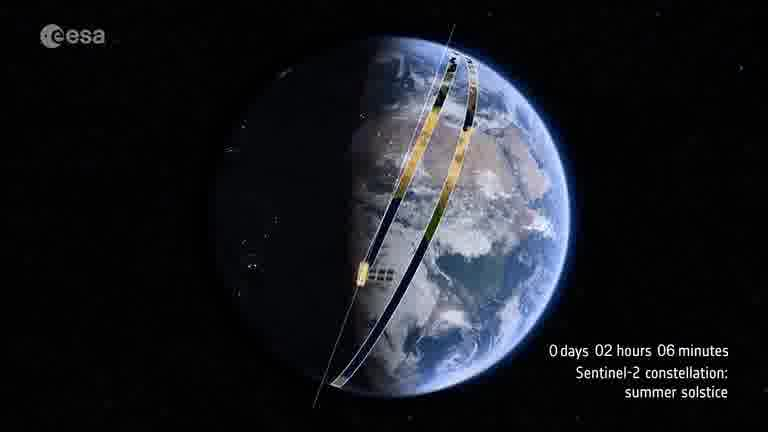
\includegraphics[width=\textwidth]{images/s2orbits/19}}
\only<3>{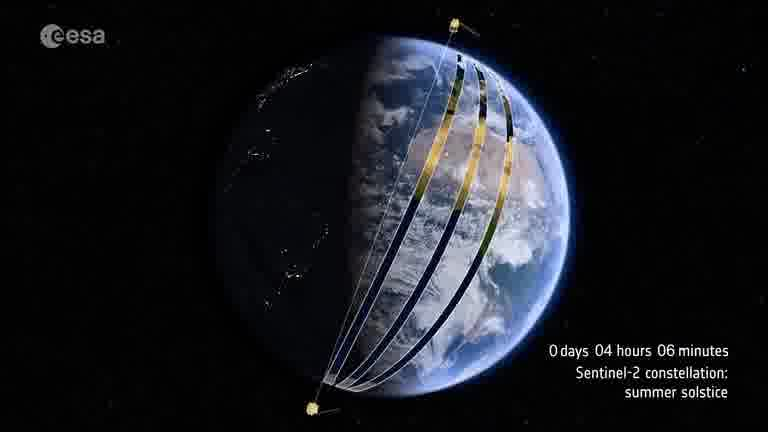
\includegraphics[width=\textwidth]{images/s2orbits/24}}
\only<4>{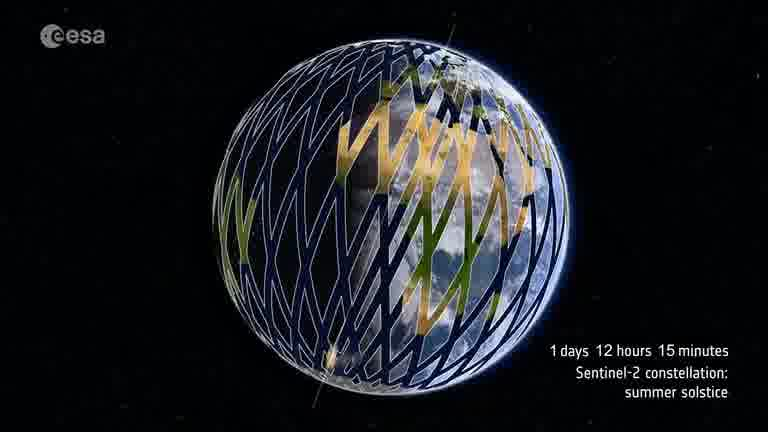
\includegraphics[width=\textwidth]{images/s2orbits/35}}
\only<5>{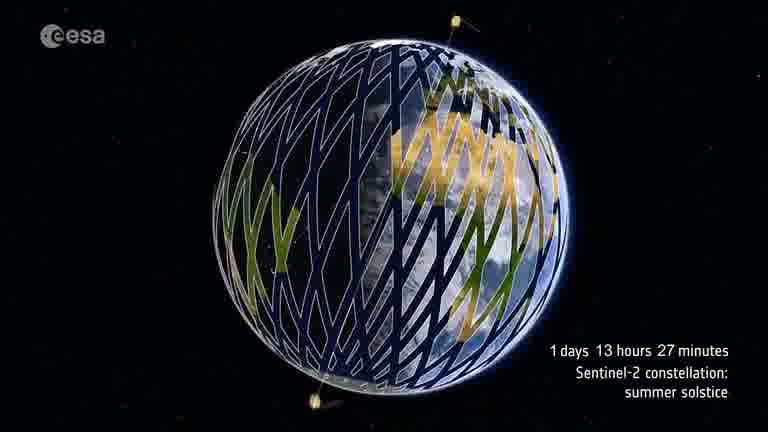
\includegraphics[width=\textwidth]{images/s2orbits/36}}
\only<6>{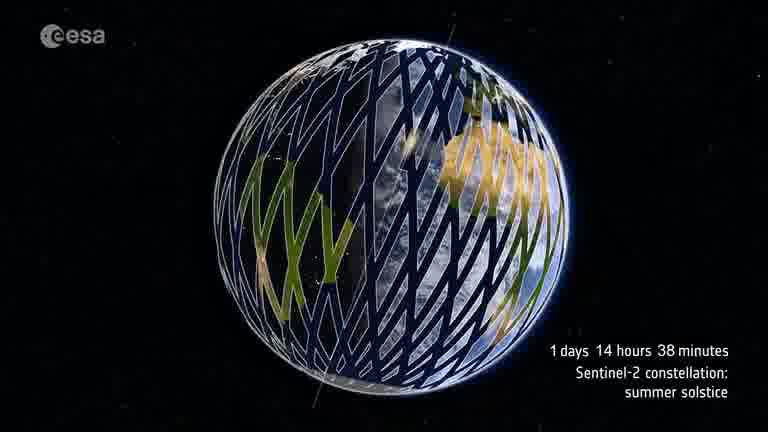
\includegraphics[width=\textwidth]{images/s2orbits/37}}
\only<7>{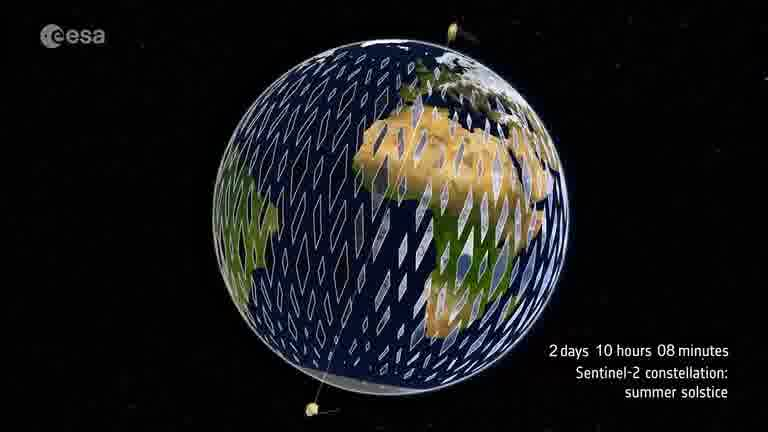
\includegraphics[width=\textwidth]{images/s2orbits/48}}
\tiny\url{https://www.esa.int/spaceinvideos/Videos/2016/08/Sentinel-2_global_coverage}
\end{columns}

\end{frame}
%
%
%{\setbeamercolor{background canvas}{bg=tumblack}
%	\begin{frame}[plain]
%	
%	\vfill
%	\Huge\color{white}
%	\begin{center}
%		\begin{columns}
%			\column{.5\textwidth}
%			\vspace{7em}
%			
%			\hfill 
%			Satellite Data Take-away
%			\column{.5\textwidth}
%			
%			
%			%%			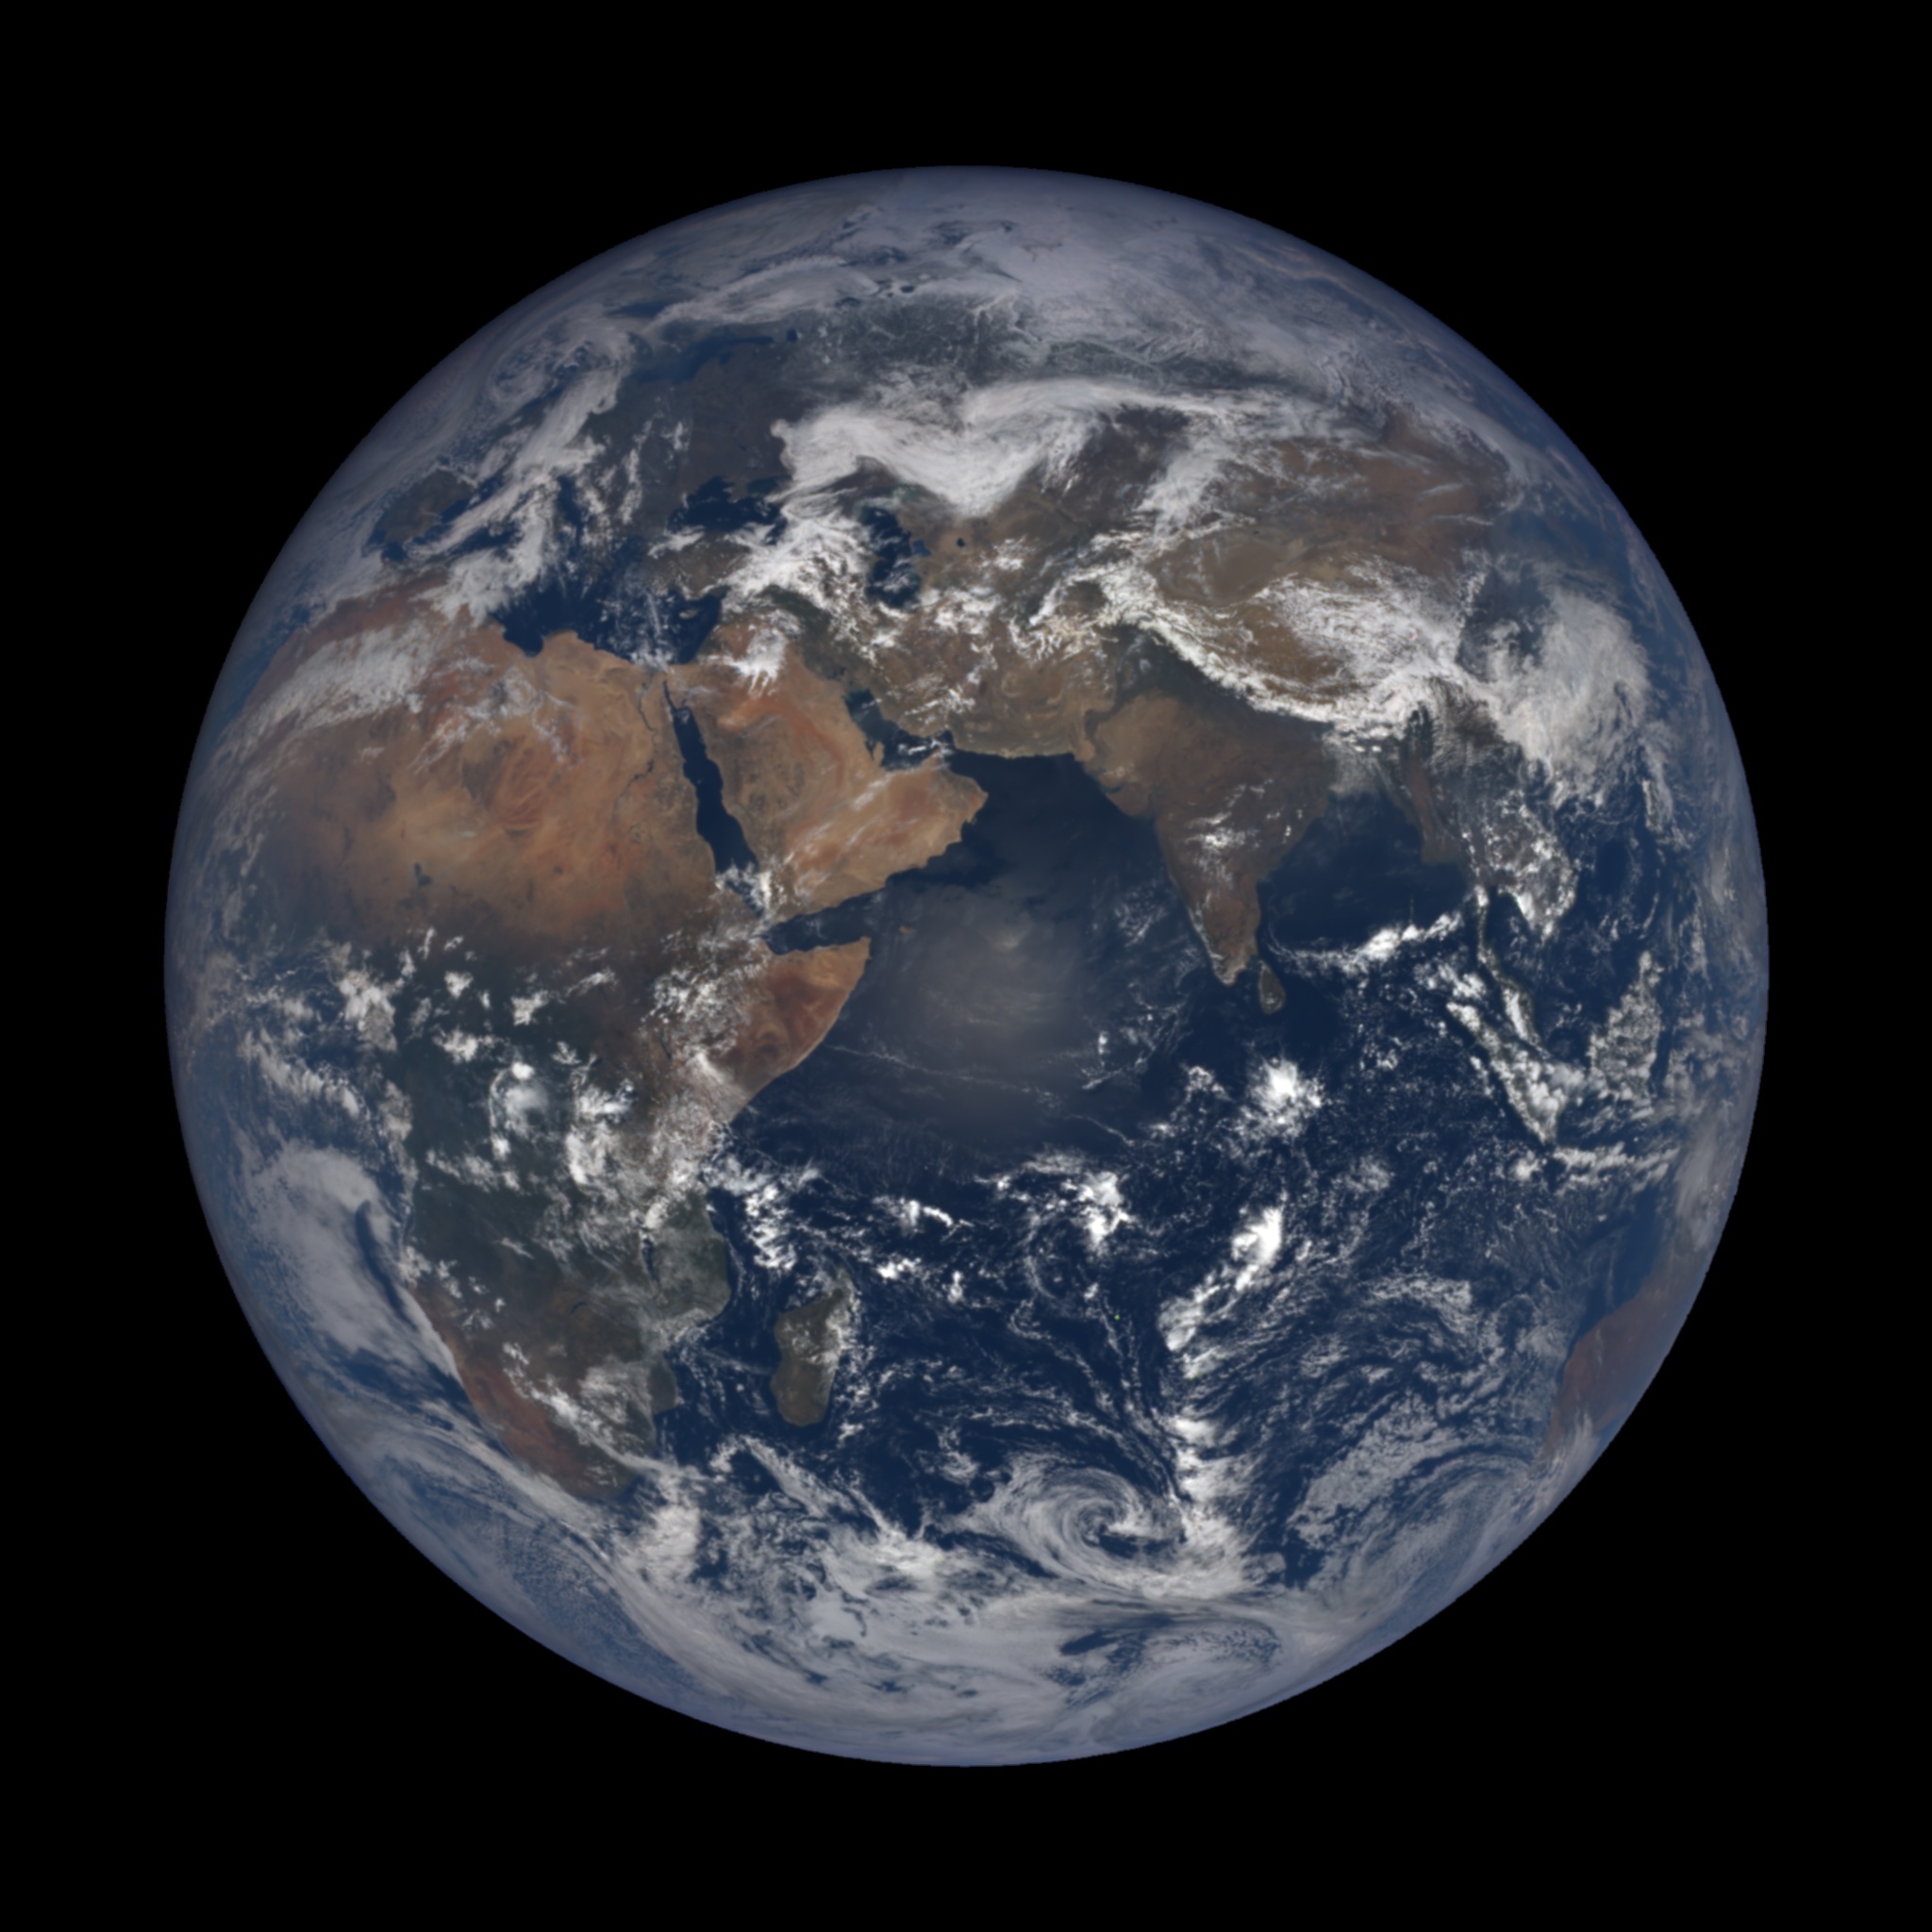
\includegraphics[width=5cm]{images/epic1}
%			%			\includegraphics[width=7cm]{images/fdl}
%		\end{columns}
%	\end{center}
%	
%	\vfill
%\end{frame}
%}

{\setbeamercolor{background canvas}{bg=tumbluedark}
\begin{frame}[plain]

\vfill
\Huge\color{white}
\begin{center}
\begin{columns}
\column{.5\textwidth}
\vspace{7em}

\hfill 
Vegetation Modeling
\column{.5\textwidth}


\includegraphics[width=\textwidth]{images/Large1954_cerial_growth_stages_white}
%%			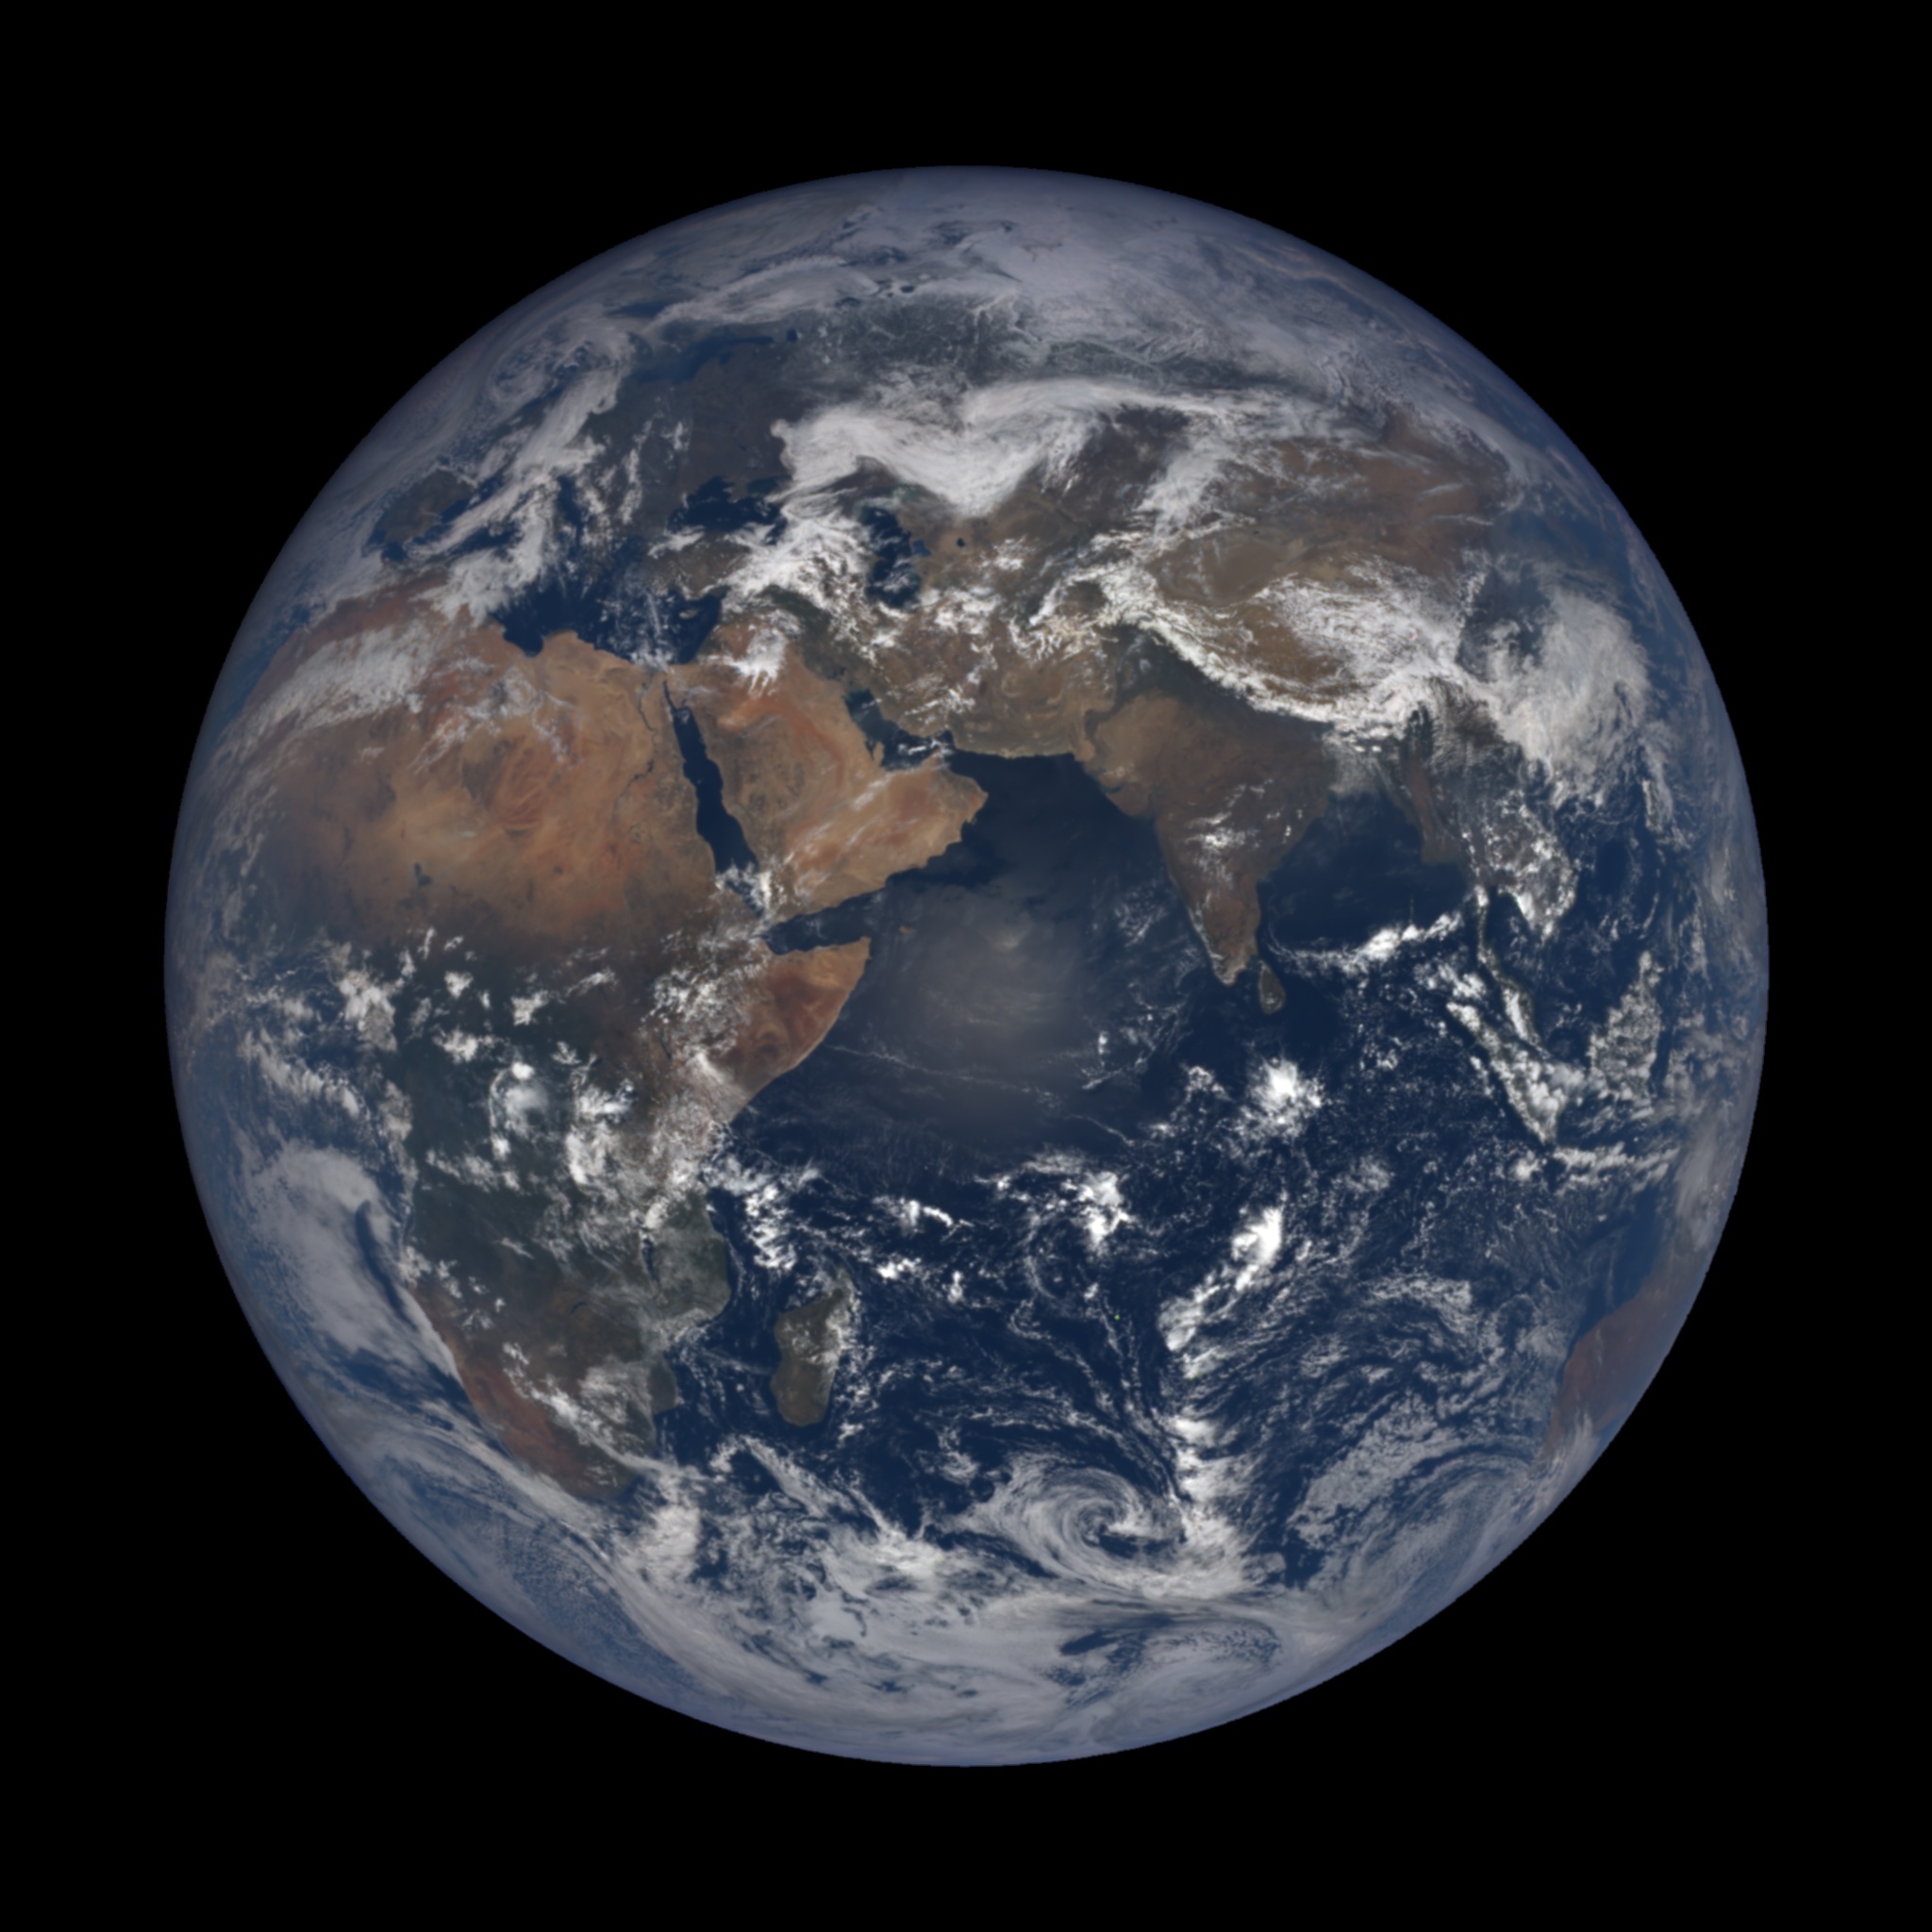
\includegraphics[width=5cm]{images/epic1}
%			\includegraphics[width=7cm]{images/fdl}
\end{columns}
\small\raggedleft(Large et al., 1954)
\end{center}

\vfill
\end{frame}
}

\begin{frame}

\frametitle{Photosynthesis}
%	
%	Photosynthesis

\centering
\begin{tikzpicture}
\node(in){$6{\text{CO}}_{2}+6{\text{H}}_{2}\text{O}$};
\node[right=of in, label={light absorbtion $\Delta \V{x}$}](arrow){$\to$};
\node[right=of arrow]{${\text{C}}_{\text{6}}{\text{H}}_{\text{12}}{\text{O}}_{\text{6}}+{\text{6O}}_{\text{2}}$};
\end{tikzpicture}
%	
%	\begin{equation*}
%	6{\text{CO}}_{2}+6{\text{H}}_{2}\text{O}\to 
%	\end{equation*}
\end{frame}


\newcommand{\rastergrid}{
\begin{tikzpicture}
% each layer
\begin{scope}[scale=2]

% raster size
\def\d{0.7}		

% distance layer
\def\s{\d*5}

\foreach \i in {1,...,6}
{		
\begin{scope}[
yshift=\s*\i,every node/.append style={
yslant=0.5,xslant=-1},yslant=0.5,xslant=-1
]
%\draw[step=3.33mm] (0,0) grid (1,1);
%\fill[black,fill opacity=.9] (0.333,0.333) rectangle (0.333,0.333);    	    	  

\foreach \row in {0,...,2}{
\foreach \col in {0,...,2}{
\draw[tumblack, fill=tumblue!\pdfuniformdeviate 40,fill opacity=1,rounded corners=1] (\col*\d/3,\row*\d/3) rectangle (\col*\d/3+\d/3, \row*\d/3+\d/3);
%                 \draw[black, fill=black!\pdfuniformdeviate 40,fill opacity=1,rounded corners=1] (\col*\d/3,\row*\d/3) rectangle (\col*\d/3+\d/3, \row*\d/3+\d/3);
}
}

%\draw[step=3.33mm] (0,0) grid (1,1);
%\fill[white,fill opacity=.9] (0,0) rectangle (1,1);
\end{scope}
}
\end{scope}
\end{tikzpicture}
}


%\begin{frame}
%\frametitle{Spectral Band}
%\end{frame}


\begin{frame}
\frametitle{Multi-temporal Vegetation Modeling}

\begin{columns}
\column{.5\textwidth}

\begin{tikzpicture}
\node[] at (0,0){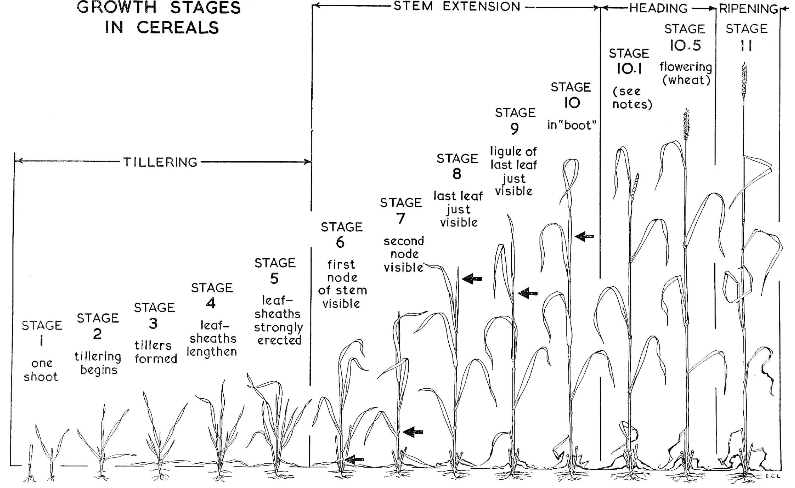
\includegraphics[width=\textwidth]{images/Large1954_cerial_growth_stages}};

%		\draw[step=1.0,black,thin, fill=none] (-2,-2) grid (2,2);

\visible<-1>{\draw [fill=white, draw=none, opacity=0.8] (-0.8,-3) rectangle (2,2.5);}
\visible<-2>{\draw [fill=white, draw=none, opacity=0.8] (2,-3) rectangle (5,2.5);}

\visible<1>{\node[rotate=190] at (-2.5,1.5){
\includegraphics[width=15mm]{images/icons/sat2}};}
\visible<2>{\node[rotate=225] at (-2.5,1.5){
\includegraphics[width=15mm]{images/icons/sat2}};}
\visible<3->{\node[rotate=260] at (-2.5,1.5){
\includegraphics[width=15mm]{images/icons/sat2}};}


%	\visible<4->{\node at (-1.5,1.4) {
\includegraphics[width=10mm]{images/cloud}};
%	}

\end{tikzpicture}

\column{.5\textwidth}

{\Large
\only<1>{
\begin{equation*}
f_\text{vegetation}(\V{X}_t)
\end{equation*}
}
\only<2>{
\begin{equation*}
f_\text{vegetation}(\V{X}_t,\V{X}_{t+1})
\end{equation*}
}
\only<3>{
\begin{equation*}
f_\text{vegetation}(\V{X}_t,\V{X}_{t+1},\V{X}_{t+2})
\end{equation*}
}
}


\vspace{2em}


\visible<1->{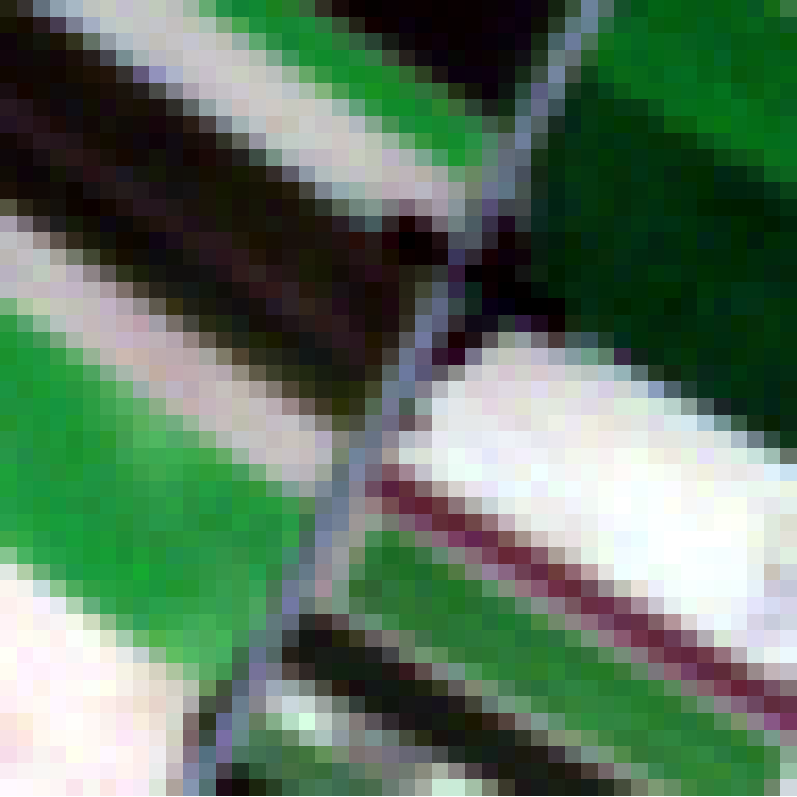
\includegraphics[width=.22\textwidth]{images/s2grid/1}}
\visible<2->{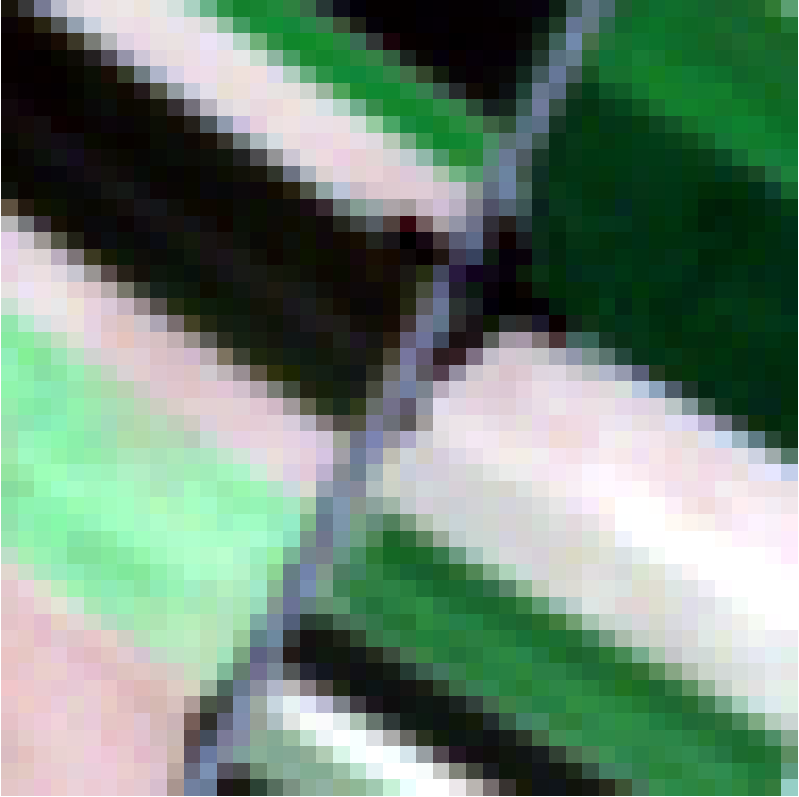
\includegraphics[width=.22\textwidth]{images/s2grid/2}}
\visible<3->{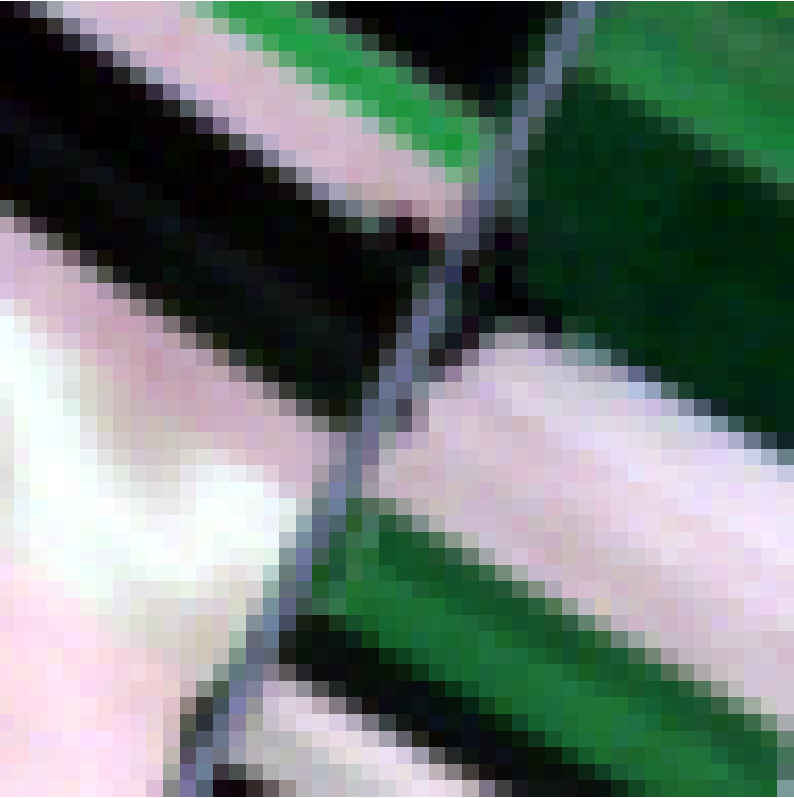
\includegraphics[width=.22\textwidth]{images/s2grid/3}}
%	\visible<4->{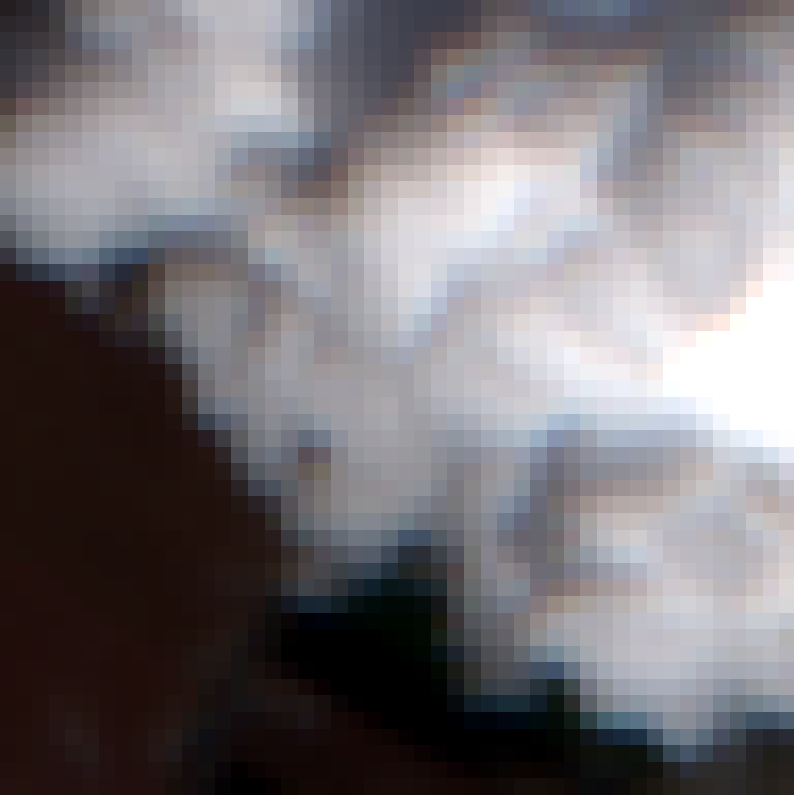
\includegraphics[width=.22\textwidth]{images/s2grid/4}}

\vspace{1em}

{\small 
Large, E. C. (1954). Growth stages in cereals illustration of the Feekes scale. Plant pathology, 3(4), 128-129.
}


\end{columns}
\end{frame}

\begin{frame}
\frametitle{Problem Definition}
\Large


\centering\begin{tikzpicture}[node distance=0em]
\visible<2->{\node(y){\V{y}};}
\visible<2->{\node[right=of y](equals){$=$};}
\node[right=of equals](f){$f_\text{vegetation}$};
\visible<1->{\node[right=of f](x){$(\V{X}_t,\V{X}_{t+1},\V{X}_{t+2})$};}

\end{tikzpicture}

\vspace{1em}
\raggedright

\begin{description}\setlength\itemsep{1em}
\item[\color{tumblue}Problem:]<1-> \textbf{unsupervised learning} of a vegetation model \textbf{is difficult}
\item[\color{tumblue}Solution:]<2-> re-framing as \textbf{supervised classification} of crop type labels
\item[\color{tumblue}Intuition:]<3-> A \textbf{supervised classification model} must \textbf{internalize} a learned \textbf{discriminative model} for the \textbf{vegetation}
\end{description}

\end{frame}

%\tikzsetnextfilename{input}

\newcommand{\timeseries}[1]{
\begin{tikzpicture}[baseline=-.25em]
	
	\tikzstyle{annot} = [font=\small\sffamily, text=tumblue]
	\tikzstyle{point} = [thin, tumbluelight, shorten >= .25em, shorten <= .25em]
	
	% from /home/marc/projects/EV2019/images/example/tstop.txt
%	\def\tstopv{0.6285714285714286}
	\def\class{winter barley}
	
	\begin{groupplot}[
	group style={
		group name=my plots,
		group size=1 by 1,
		columns=1,
		xlabels at=edge bottom,
		xticklabels at=edge bottom,
		vertical sep=1em,
	},
	ylabel near ticks,
	ylabel style={font=\sffamily\small, rotate=-90},
	width=.75\textwidth,
	height=3.8cm,
	axis x line=bottom,
	axis y line=left,
	enlarge x limits=0.01,
	xtick={0,0.25,0.5,0.75,1},
	xticklabels={Januar,April,Juni,September,Dezember},
	ymajorgrids,
	ymin=0, ymax=1.4
	]
	
	
	
	\nextgroupplot[
		no marks,  
		ylabel={},
		draw opacity=.8,
		smooth=0.01,
		legend columns=2,
		legend style={at={(.5,1.1)},anchor=south, line width=1pt, fill=tumblue!10}
		]
		 
	\addplot[b1color] table [x=t, y=B1, col sep=comma, forget plot] {images/example/#1};
	\addplot[b9color] table [x=t, y=B9, col sep=comma, forget plot] {images/example/#1};
	\addplot[b10color] table [x=t, y=B10, col sep=comma] {images/example/input.csv};
	
	\addplot[b11color] table [x=t, y=B11, col sep=comma, forget plot] {images/example/#1};
	\addplot[b12color] table [x=t, y=B12, col sep=comma] {images/example/#1};
	
	\addplot[b5color] table [x=t, y=B5, col sep=comma, forget plot] {images/example/#1};
	\addplot[b6color] table [x=t, y=B6, col sep=comma, forget plot] {images/example/#1};
	\addplot[b7color] table [x=t, y=B7, col sep=comma, forget plot] {images/example/#1};
	\addplot[b8color] table [x=t, y=B8, col sep=comma, forget plot] {images/example/#1};
	\addplot[b8Acolor] table [x=t, y=B8A, col sep=comma] {images/example/#1};
		
	\addplot[b2color] table [x=t, y=B2, col sep=comma, forget plot] {images/example/#1};
	\addplot[b3color] table [x=t, y=B3, col sep=comma, forget plot] {images/example/#1};
	\addplot[b4color] table [x=t, y=B4, col sep=comma] {images/example/#1};
%	
	\legend{3 atmospheric, 2 short-wave infrared, 5 near infrared, 3 visible bands}
	
%	\addplot[thick,colorclassone, name path=y1] table[x=t, y=y1]{\mydata};
%	\addplot[thick,colorclasstwo, name path=y2] table[x=t, y=y2]{\mydata};
%	\addplot[thick,colorclassthree, name path=y3] table[x=t, y=y3]{\mydata};
%	\addplot[thick,colorclassfour, name path=y4] table[x=t, y=y4]{\mydata};
	%\addplot[colorblue!20] fill between[of = y1 and axis];
	%\addplot[colorhgray!20] fill between[of = y2 and axis];
	%\addplot[colorgreen!20] fill between[of = y3 and axis];
	%\addplot[colororange!20] fill between[of = y4 and axis];
	
	
	\end{groupplot}
	
	\end{tikzpicture}
}

\begin{frame}
\frametitle{Crop Type Labels in Europe}

\begin{columns}

\column{.5\textwidth}

\Large

\begin{description}\setlength\itemsep{1em}
\item[\color{tumblue}collected] yearly within European \textbf{Common Agricultural Policy} (CAP)
\item[\color{tumblue}declared] by Farmers at \textbf{crop subsidy} applications
\item[\color{tumblue}today] slowly made publicly available (on a national basis)
\item[\color{tumblue}in future] further harmonized within \textbf{Europe's INSPIRE} directive
\end{description}

\column{.5\textwidth}
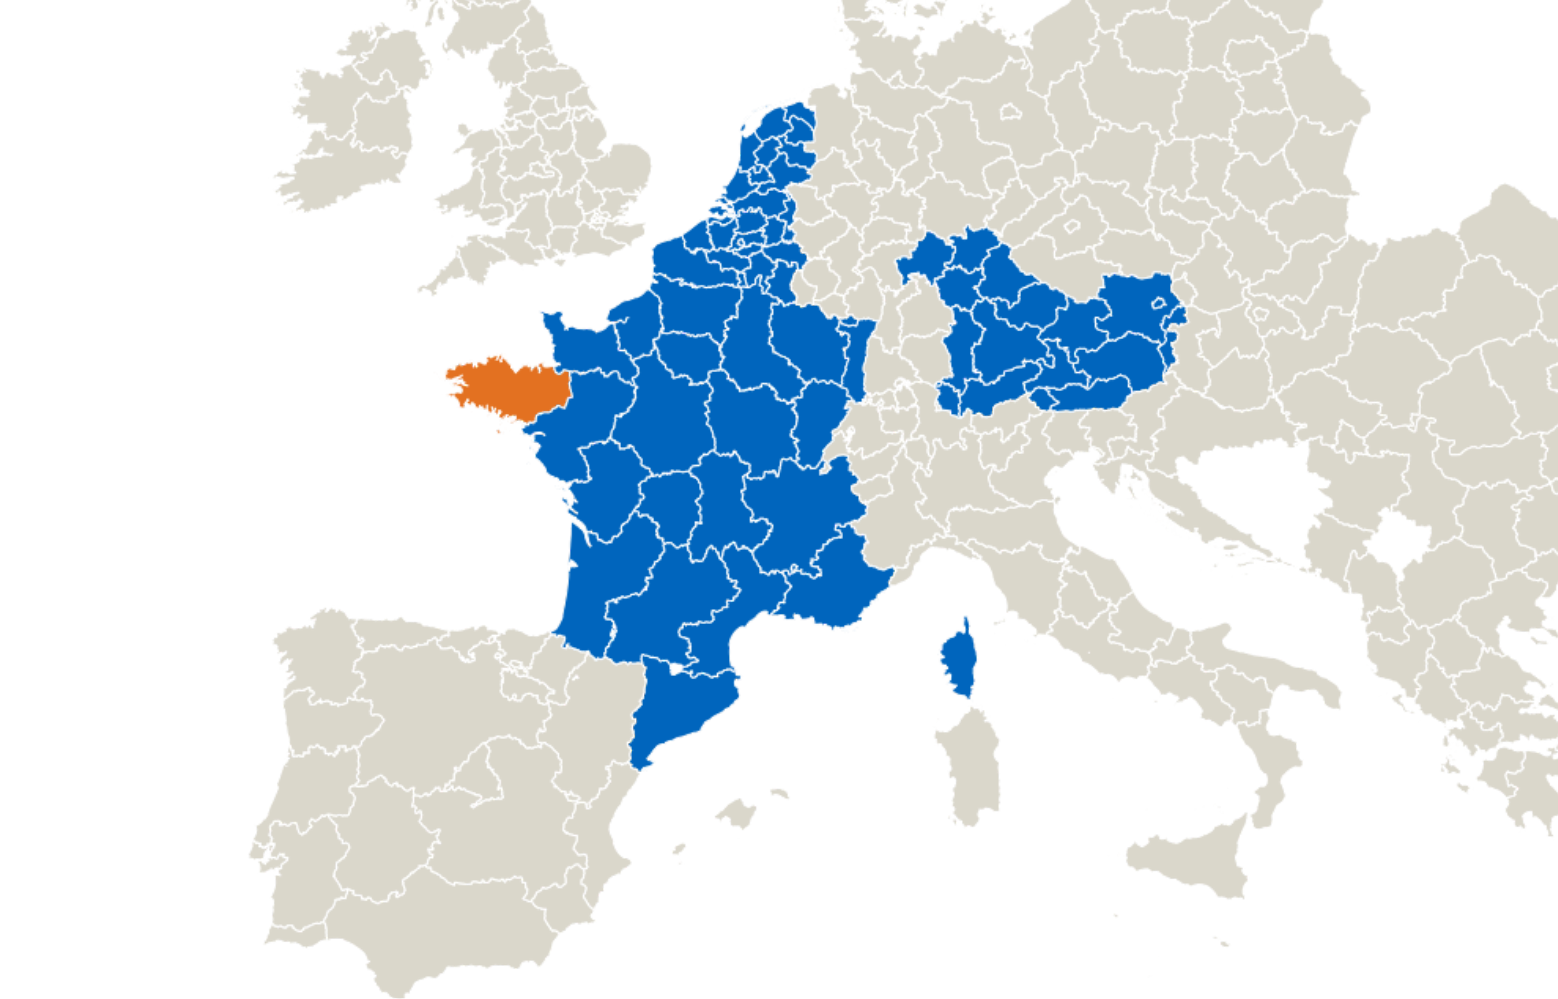
\includegraphics[width=\textwidth]{images/europe_data2}


\end{columns}
\end{frame}



\begin{frame}
\frametitle{Projects}

\begin{itemize}
	\item supervised crop type mapping
	\item early classification
\end{itemize}

\end{frame}

\begin{frame}
	\frametitle{Outlook and Directions}
	\begin{itemize}
		\item away from strict supervised learning
		\item large scale dataset creation
		\item domain transfer between regions
		\item vegetation modeling
	\end{itemize}
\end{frame}

\end{document}



